\chapter{Universal Gravitation}
\label{chapter:gravity}


  
\section{Law of Universal Gravitation}
\begin{figure}[ht]
  \centering
  \begin{tikzpicture}[scale=.65]
    \draw[vector,red] (0,0)--(2,0) node[right]{$\bm F_{21}$};
    \draw[vector,blue] (8,0)--(6,0) node[left]{$\bm F_{12}$};
    \shade[ball color=red] circle (.7) node[white]{$m_1$};
    \shade[ball color=blue] (8,0) circle (1)  node[white]{$m_2$};
    \draw[dashed] (0,0)--(0,-1.5);
    \draw[dashed] (8,0)--(8,-1.5);
    \draw[axes] (0,-1.3)--(8,-1.3) node[midway,below]{$\bm r_{12}$};
  \end{tikzpicture}
  \caption{Gravitational attraction between two point masses.}
  \label{fig:grav-force}
\end{figure}
In classical mechanics, \textbf{gravity} is a mutually attractive force
between massive objects (shown in Fig.~\ref{fig:grav-force}). The magnitude of
the gravitational force is given by the \textbf{law of universal
  gravitation}\footnote{We now know that the ``law'' of ``universal''
gravitation is neither a law nor is it universal. The law fails near extremely
massive objects like black holes and neutron stars, and must be replaced with
general relativity. For extremely small masses, like electrons and protons, it
is not known whether the law applies. We also know that in general relativity,
gravitation is not an actual force, but the rather, the result of
curvature in spacetime.}:
\begin{equation}
  \boxed{
    F_g=\frac{Gm_1m_2}{r^2}
  }
  \label{eq:universal-grav}
\end{equation}
where $G=\SI{6.674e-11}{\newton.\metre\squared\per\kilo\gram\squared}$ is the
\textbf{universal gravitational constant}, $r$ is the distance between the
masses. In this equation, $m_1$ and $m_2$ are \emph{point masses} that do not
occupy any space. By the third law of motion: If $m_1$ exerts a gravitational
force $\bm F_{12}$ on $m_2$, then $m_2$ likewise also exerts a reaction force of
$\bm F_{21}=-\bm F_{12}$ on $m_1$. The two forces are equal in magnitude and
opposite in direction, hence the attraction is \emph{mutual}.

\begin{common-question}
  \textbf{What happens when $r=0$?} It is worth pointing out that point masses
  do not actually exist, and that even an electron has a finite size. Therefore
  the situation for $r=0$ will never arise; $F_g$ can never be infinite. From a
  practical point of view, whether a mass can be treated as a point mass is a
  matter of \emph{scale}. For example, at the scale of the solar system, the
  sun and all the planets, moons, comets can all be considered as point masses,
  but at the surface of an irregularly-shaped asteroid, the point mass model
  would be very inaccurate.
\end{common-question}

For a mass subjected to the influence of multiple discrete point masses $m_i$,
say, for example. in Fig.~\ref{fig:multiple-masses}),
\begin{figure}[t]
  \centering
  \begin{tikzpicture}[scale=.4]
    \shade[ball color=red] circle (.7) node[white]{$M$};

    \draw[vector,blue,rotate=45] (.7,0)--(2.5,0) node[right]{$\bm F_1$};
    \shade[ball color=blue] (5,5) circle (.8) node[white]{$m_1$};

    \draw[vector,green,rotate=-45] (-.7,0)--(-2,0) node[left]{$\bm F_2$};
    \shade[ball color=green] (-5,5) circle (.6) node[white]{$m_2$};

    \draw[vector,violet,rotate=45](-.7,0)--(-3.5,0) node[left]{$\bm F_3$};
    \shade[ball color=violet] (-5,-5) circle (1.2) node[white]{$m_3$};

    \draw[vector,magenta,rotate=-45](.7,0)--(2.7,0) node[right]{$\bm F_4$};
    \shade[ball color=magenta] (5,-5) circle (.8) node[white]{$m_4$};
  \end{tikzpicture}
  \caption{A mass that is subjected to multiple gravitational forces}
  \label{fig:multiple-masses}
\end{figure}
the total gravitational force that $M$ experiences is the vector sum of all
the forces $\bm F_i$:
\begin{equation}
  \boxed{
    \bm F=\sum_i\bm F_i
    =-GM\left[\sum_{i=1}^N\frac{m_i}{r_i^2}\hat{\bm r_i}\right]
  }
\end{equation}
where $r_i$ is the distance from $M$ to $m_i$, and $\hat{\bm r_i}$ is the
outward radial direction from $m_i$ towards $M$.

At the limit $N\rightarrow\infty$, the summation becomes an integral, and can
now be used to describe the gravitational force from objects with
\emph{spatial extend} i.e.\ masses that take up space (e.g.\ a continuous
distribution of mass):
\begin{equation}
  \bm F=-\int\dl{\bm F}=-GM\int\frac{\dl m}{r^2}\hat{\bm r}
\end{equation}
where $\hat{\bm r}$ is the outward radial direction from $\dl m$ towards $M$.
Objects that are symmetrically spherical (e.g.\ planets are stars in our
solar system) can be treated as point masses, and integration can be avoided.
However, this is not always the case.



\section{Gravitational Field}
As seen in Chapter~\ref{chapter:dynamics}, we generally describe the
gravitational force acting on any mass $m$ (i.e.\ its weight) as:
\begin{equation*}
  \bm F_g=m\bm g
\end{equation*}
where $\bm g$ is the acceleration due to gravity at the location of $m$.
This equation is always
correct as long as we have the correct magnitude and direction of $\bm g$.
But in light of our new knowledge of the law of universal gravitation in
Eq.~\ref{eq:universal-grav}, to find the gravitational force on $m_2$ in a
two-mass system, we can group the variables in the law of universal
gravitation to find $\bm g$:
\begin{equation*}
  F_g
  =\underbracket[1pt]{\left[\frac{Gm_1}{r^2}\right]}_{=g}m_2
  =m_2 g
\end{equation*}
The vector field function $\bm g$ is known as the \textbf{gravitational field}
generated by point mass $m_1$. It is a function of the magnitude of the source
mass $m_s$, and the distance $r$ from it:
\begin{equation}
  \boxed{
    \bm g(m_s,\bm r)=-\frac{Gm_s}{r^2}\hat{\bm r}
  }
  \label{eq:g}
\end{equation}
The direction of the gravitational field is the inward radial direction
$-\hat{\bm r}$, i.e.\ $\bm g$ points towards the source mass. The gravitational
field function shows how a mas influences the gravitational forces on other
masses in its vicinity. On/near the surface of Earth, we can substitute the
mass and radius of Earth ($m_s=m_E=\SI{5.972e24}{\kilo\gram}$ and
$r=r_E=\SI{6.371e6}\metre$) to obtain the commonly-known value of
\begin{equation*}
  g\approx\SI{9.81}{\metre\per\second\squared}\quad\text{or}\quad
  g\approx\SI{9.81}{\newton\per\kilo\gram}
\end{equation*}
Both units are equivalent.



\subsection{Gravitational Fields from Multiple Masses}
When multiple discrete points are present, the total gravitational
field at any point of interest is the vector sum of all the fields $\bm g_i$
from those masses:
\begin{equation}
  \boxed{\bm g
    =\sum_i\bm g_i
    =-G\left[\sum_{i=1}^N\frac{m_i}{r_i^2}\hat{\bm r}_i\right]
  }
\end{equation}
where $r_i$ is the distance from the point of interest to $m_i$ and $\hat{\bm r}_i$
is the direction from the discrete mass $m_i$ towards the point of interest.

As $N\rightarrow\infty$, the summation becomes an integral, and we can use it
now be used to describe the gravitational field generated by objects with
\emph{spatial extend} (i.e.\ continuous distribution of mass):
\begin{equation}
  \boxed{
    \bm g
    =\int\dl{\bm g}
    =-G\int\frac{\dl m}{r^2}\hat{\bm r}
  }
\end{equation}
where $\hat{\bm r}$ is the outward radial direction from $\dl m$ towards the point
of interest. This integral may be difficult to compute if the geometry is complicated.

%When a mass $m$ is placed inside a gravitational field $\bm g$, it
%experiences a gravitational force given by the familiar equation:
The gravitational field $\bm g$ doesn't \emph{do} anything itself, until another mass
$m$ is placed inside the field. Then, the gravitational field applies a  force
$\bm F_g$ on that mass $m$, given by the familiar equation:
  %enters the field. Then, $m$ experiences a gravitational force 
  %proportional to $m$ and $\bm g$, 
\begin{equation*}
  \bm F_g=m\bm g
\end{equation*}
The direction of the force is the same as the gravitational field. This equation
applies regardless of how the field is created.

The concept of the gravitational field separates the force problem into to parts:
\begin{enumerate}[nosep]
\item The creation of the gravitational field, and
\item The effects of that gravitational field, which is always $\bm F_g=m\bm g$
\end{enumerate}
In the example in Fig.~\ref{fig:g-example1}:
\begin{itemize}
\item The masses $m_1$ and $m_2$ generate gravitational fields
  $\bm g_1$ and $\bm g_2$. The gravitational fields extend throughout space, and
  both point towards the source. Far from these masses, $m_1$ and $m_2$ can be treated
  as point masses, and the gravitational fields are given by equation Eq.~\ref{eq:g}.
\item At position $P$, the total field is the vector sum of both masses, i.e.
  $\bm g_\text{tot}=\bm g_1+\bm g_2$. At this point,
  there is nothing at $P$, and the gravitational field does not do anything.
\item When a mass $m$ is placed inside the gravitational field, it experiences a
  gravitational force of $\bm F_g=m\bm g_\text{tot}$. The force is in the same
  direction as $\bm g_\text{tot}$.
\item Since the gravitational field is also the acceleration due to gravity, if 
  gravity is the only force acting on $m$, its acceleration at $P$ would be
  $\bm a=\bm g_\text{tot}$. If gravity is not the only force, then the mass's
  acceleration would be based on the second law of motion.
\end{itemize}
\begin{figure}[ht]
  \centering
  \begin{tikzpicture}
    \node at (0,0) {\pic{.05}{universalGravitation/Earth-planet}};
	\draw[violet] circle (.4) node[white]{$\bm m_1$};
    \foreach \theta in {0,30,...,359}{
      \draw[vector,violet,rotate=\theta] (2,0)--(1,0);
      \draw[very thick,violet,rotate=\theta] (3,0)--(.4,0);
    } 
    \node at (-10,2) {\pic{.03}{universalGravitation/moon}};
	\draw[orange] (-10,2) circle (.25) node[orange]{$\bm m_2$};
    \foreach \theta in {0,30,...,359}{
      \draw[vector,orange,rotate around={\theta:(-10,2)}] (-8,2)--(-9,2);
      \draw[very thick,orange,rotate around={\theta:(-10,2)}] (-7,2)--(-9.75,2);
    }   
    \draw[vector,violet,rotate around={-45:(-4,4)}] (-4,4)--+(1.8,0)
    node[right]{$\bm g_1$};
    \draw[vector,orange,rotate around={atan(2/6):(-4,4)}] (-4,4)--+(-.9,0)
    node[left]{$\bm g_2$};
    \fill (-4,4) circle (.08) node[above]{$P$};
  \end{tikzpicture}
  \caption{Gravitational field from two masses}
  \label{fig:g-example1}
\end{figure}
In this example, we have looked at a specific point $P$, but
ultimately, our goal would be to describe the gravitational field generally,
i.e.\ as $\bm g(\bm x,t)$ for every position $\bm x$ in a space that we are
interested in. If this function is available, we do not have to consider
\emph{how} the field is generated in the first place.



\subsection{Spherical Shell}

\begin{figure}[ht]
  \centering
  \begin{tikzpicture}[scale=.45]
    \draw[thick,fill=gray] circle (5) node[above]{$m_1$};
    \draw[thick,fill=white] circle (4.9);
    \draw[axes,rotate=30] (0,0)--(4.9,0) node[midway,below]{$R$};
    \draw[mass] (1,-1) circle (.2) node[below]{$m_2$};
  \end{tikzpicture}
\end{figure}
Newton used the \textbf{shell theorem} to show that if a mass $m_2$ is
\emph{inside} a spherical shell of mass $m_1$, the gravitational force that
it experiences is \emph{zero}.
\begin{equation}    
  \boxed{
    \bm F_g=
    \begin{cases}
      \bm 0 & \text{if}\;\;r<R\\
      -Gm_1m_2/r^2\hat{\bm r} & \text{otherwise}
    \end{cases}
  }
\end{equation}
It also means that gravitational field is also \emph{zero} inside the shell.
That $\bm g_\text{inside}=\bm 0$ can be calculated by integrating the fields
created by infinitesimal mass elements $\dl m$ at any point inside the shell,
or use a form of \textbf{Gauss's law} for gravity, similar the equation to
find the electric field inside a charged conducting sphere:
\begin{equation}
  \oint\bm g\cdot\dl{\bm A}=-4\pi GM_\text{encl}
\end{equation}
Gauss's law is studied in further detail for \emph{electric} fields in
Chapter~\ref{chapter:gauss}\footnote{As a quick reference, Gauss's law for
electricity is stated as:
\begin{equation*}
  \oint_\mathcal{S}\bm E\cdot\dl{\bm A}=\frac{q_\text{encl}}{\epsilon_0}
\end{equation*}
Since gravitational and electric fields share many similarities, we can adapt
it for gravitational field as well All we have to do is to replace electric
field $\bm E$ with gravitational field $\bm g$, enclosed charge $q_\text{encl}$
with enclosed mass $M_\text{encl}$ and the permittivity of free space
$\epsilon_0$ with $\dfrac1{4\pi G}$.}.

The gravitational field strength inside spherical shell is shown in
Fig.~\ref{fig:spherical-shells}.
\begin{figure}[ht]
  \centering
  \begin{tikzpicture}
    \draw[axes] (0,0)--(0,3) node[above]{$|\bm g|$};
    \draw[axes] (0,0)--(5.5,0) node[right]{$r$};
    \draw[thick,dashed] (1,0)--(1,2) node[pos=0,below]{$R$}--(0,2)
    node[left]{$\dfrac{GM}{R^2}$};
    \draw[function,samples=15,smooth,domain=1:5] plot(\x,{2/\x});
    \draw[function] (0,0)--(1,0);
    \draw[function,fill=black!2] (1,0) circle (.06);
    \fill[red!80!black] (1,2) circle (.06);
  \end{tikzpicture}
  \caption{Gravitational field strength inside and outside a spherical shell
    of radius $R$.}
  \label{fig:spherical-shells}
\end{figure}



\subsection{Uniform Spherical Mass}

\begin{figure}[ht]
  \centering
  \begin{tikzpicture}[scale=.45]
    \draw[thick,fill=gray!50] circle(5);
    \draw[thick,fill=gray!10] (-.2,5) rectangle(.2,-5);
    \draw[mass] (0,1) circle(.15) node[right,black]{$m$};
  \end{tikzpicture}
\end{figure}
Suppose you could drill a hole through the Earth and then jump into it. How
long would it take you to emerge on the other side of the Earth?

To calculate this, we need to know how the gravitational force
changes as you fall through Earth.

\begin{figure}[ht]
  \centering
  \begin{tikzpicture}
    \node at (0,0) {\pic{.32}{universalGravitation/earth-1200px}};
    \draw (-.18,2.35)--(-.18,-2.35);
    \draw (.18,2.35)--(.18,-2.35);
    \fill[gray,opacity=.8] (-.18,2.35) rectangle (.18,-2.35);
    \draw[very thick,fill=gray,opacity=.3] circle (2.35);
    \draw[dashed,very thick,fill=gray,opacity=.5] circle (1.1);
    \node at (0,1.3) {\pic{.018}{universalGravitation/falling-person}};
    \draw[axes] (3,1.7)--(.5,1.7) node[pos=0,right]{
      \scriptsize The mass above does not contribute to gravity};
    \draw[axes] (3,.5)--(.5,.5) node[pos=0,right]{
      \scriptsize The mass below contributes to gravity};
  \end{tikzpicture}
  \caption{Dividing into above and below}
\end{figure}

As you fall through Earth, we can separate the part of Earth that is
``above'' you, and the part that is ``below'' you
\begin{itemize}
\item The part that is ``above'' you is like the spherical shell, and does
  not contribute to the gravitational field, and therefore does not exert
  any force
\item The part that is ``below'' you gets smaller as you fall towards the
  centre
\end{itemize}



Assuming that Earth's density is uniform, and neglecting air resistance and
other factors, the value of $g$ as the person falls through Earth ($r<R$) is
given by finding how much mass is still ``below'' the person, $M(r)$:
\begin{equation}
  g(r)=\frac{GM(r)}{r^2}\quad\quad M(r)=\frac43\rho\pi r^3\quad\quad
  \rho=\frac{3M_E}{4\pi r_E^3}
\end{equation}
where $M_E$ is the mass of Earth, $r_E$ is the radius of Earth, $\rho$ is the
(constant) density, and $r$ is the distance from Earth's centre. Then $M(r)$
is the amount of mass ``below'' the person as he/she falls towards the centre.

The gravitational field strength inside this hypothetical Earth is a
linear function of distance $r$ from the centre:
\begin{equation}
  g(r)=\frac{GM_E r}{r_E^3}=\left(\frac r{r_E}\right)g_0
\end{equation}
where $g_0=\SI{9.81}{\newton\per\kilogram}$ is the field strength at Earth's
surface, and $r_E=\SI{6371}{\kilo\metre}$ is Earth's radius. The gravitational
field strength inside and outside a uniform sphere is shown as a function
distance $r$ from the centre of the sphere in Fig.~\ref{fig:g-sphere}.
\begin{figure}[ht]
  \centering
  \begin{tikzpicture}
    \draw[axes] (0,0)--(0,3) node[above]{$|\bm g|$};
    \draw[axes] (0,0)--(5.5,0) node[right]{$r$};
    \draw[thick,dashed] (1,0)--(1,2) node[pos=0,below]{$R$}--(0,2)
    node[left]{$\dfrac{GM}{R^2}$};
    \draw[function,domain=1:5] plot(\x,{2/\x});
    \draw[function] (0,0)--(1,2);
  \end{tikzpicture}
  \caption{Gravitational field strength inside and outside a uniform sphere
    of radius $R$.}
  \label{fig:g-sphere}
\end{figure}
The gravitational field strength is zero at the centre inside the sphere, and
the increases linearly to the surface $r=R$, then drops off as $1/r^2$ outside
the sphere.

The gravitational force is the falling mass times the gravitational field:
\begin{equation}
  F_g(r)=-mg=-\left[\frac{mg_0}{r_E}\right] r
\end{equation}
%The fact that gravitational field scales linearly with $r$ presents an
%interesting situation.
Any mass inside the sphere will experience a force that is proportional to the
distance $r$ from the centre, and in the opposite direction from the
displacement from the centre. This means that gravitational force has the same
form as Hooke's law: it is proportional to displacement from the centre, but in
the opposite direction:
\begin{equation}
  F_g(r)=-kr \quad\text{where}\quad k=\frac{mg_0}{r_E}
\end{equation}
The resulting motion is a simple harmonic motion, with a natural frequency of:
\begin{equation}
  \omega_0=\sqrt{\frac km}=\sqrt{\frac{g_0}{r_E}}
\end{equation}
The traveller will therefore oscillate through Earth with a period of:
\begin{equation}
  T=\frac{2\pi}{\omega_0}=2\pi\sqrt{\frac{r_E}{g_0}}
\end{equation}
For Earth, $T=\SI{5068}\second$. The traveller would pop up on the opposite
side every 42 minutes. Since simple harmonic motion is a projection of a
uniform circular motion, if a satellite is in a circular orbit just above the
surface, and passes overhead just above the traveller as he/she popped up out
of the hole. The period of such an orbit would be the same as oscillating
traveller (Fig.~\ref{fig:withsatellite}).
\begin{figure}[ht]
  \centering
  \begin{tikzpicture}
    \node at (0,0) {\pic{.32}{universalGravitation/earth-1200px}};
    \fill[gray!50,opacity=.5] (-.18,2.35) rectangle (.18,-2.35);
    \draw[very thick] circle (2.35);
    \draw[dashed,very thick,lightgray] circle (2.55);
    \foreach\theta in {5,50,95,140,185}{
      \draw[vector,red,rotate=\theta] (0,2.55) arc(90:105:2.55);
    }
    \node[rotate=-30] at (0,2.5) {
      \pic{.05}{universalGravitation/6856-small.png}};
    \node[rotate=-210] at (0,-2.5) {
      \pic{.05}{universalGravitation/6856-small.png}};

    \draw (-.18,2.35)--(-.18,-2.35);
    \draw (.18,2.35)--(.18,-2.35);

    \node at (0,2.2) {\pic{.02}{universalGravitation/falling-person}};
    
    \draw[vector] (0,1.8)--(0,1.4);
    \draw[vector] (0,1.3)--(0,.6);
    \draw[vector] (0,.5)--(0,-.5);
    \draw[vector] (0,-.6)--(0,-1.3);
    \draw[vector] (0,-1.4)--(0,-1.9);
    \draw[vector] (0,-2)--(0,-2.3);
  \end{tikzpicture}
  \caption{A satellite travelling just above the surface of Earth has the
    same period of motion as the falling traveller.}
  \label{fig:withsatellite}
\end{figure}


\section{Gravitational Field Lines}
\begin{figure}[ht]
  \centering
  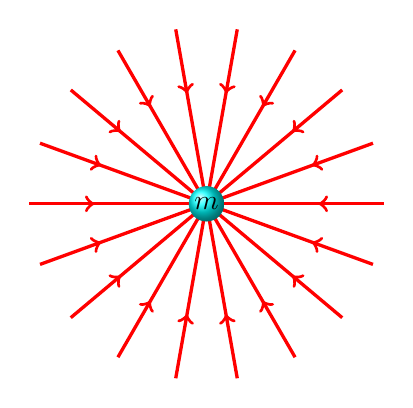
\begin{tikzpicture}[scale=1.5]
    \foreach \x in {0,20,...,359}{
      \begin{scope}[red,very thick,rotate=\x]
        \draw (0,0)--(1,0);
        \draw[<-](.95,0)--(1.5,0);
      \end{scope}
    }
    \shade[ball color=cyan] circle(.15) node{$m$};
  \end{tikzpicture}
  \caption{Gravitational field lines from a point mass.}
  \label{fig:grav-field-lines}
\end{figure}
%\begin{itemize}
%\item The direction of $\bm g$ is towards the centre of the object that
%  created it
%\item Field lines do not tell the intensity (i.e.\ magnitude) of $\bm g$,
%  only the direction
%\end{itemize}
%
%When there are multiple masses, the total gravitational field (dotted line)
%is the vector sum of all the individual fields.
%\begin{center}
%  \includegraphics[width=.4\textwidth]{universalGravitation/grav-fields}
%\end{center}
%The solid lines are called \textbf{equipotential lines}, where the potential
%energy is constant. Equipotential lines are perpendicular to
%gravitational field lines.







\section{Gravitational Potential Energy}

\textbf{Gravitational potential energy} stored between two masses is obtained
by integrating the work ($W_g$) done by the gravitational force ($\bm F_g$):
\begin{equation*}
  W_g =\int \bm F_g\cdot\dl{\bm r}
  =-\int_{r_0}^{r_1}\frac{Gm_1m_2}{r^2}\hat{\bm r}\cdot\dl{\bm r}
  =-Gm_1m_2\int_{r_0}^{r_1}\frac{\dl r}{r^2}=\frac{Gm_1m_2} r\Big|^{r_1}_{r_0}
  =-\Delta U_g
\end{equation*}
where the \textbf{gravitational potential energy} is defined as
\begin{equation} 
  \boxed{U_g=-\frac{Gm_1m_2}r}
  \label{eq:real-Ug}
\end{equation}
$U_g$ is the work required to move two objects from $r=r_0$ to $\infty$. From
this equation, $U_g\leq 0$: $U_g=0$ at $r=\infty$ and \emph{decrease} (i.e.\
becomes ``more negative'') as $r$ decreases\footnote{That $U_g$ is negative
should not bother anyone. Even when we expressed the energy as $U_g=mgh$ in
Chapter~\ref{chapter:energy}, we would often get $U_g<0$ when the object is
below the reference level (where $h=0$). Eq.~\ref{eq:real-Ug} allows us to
generalize all gravitational potential energies}. As we have already seen in
Chapter~\ref{chapter:energy}, the work done by gravity is related to the
gravitational potential energy by:
\begin{equation}
  \boxed{
    W_g=-\Delta U_g
  }
\end{equation}
indicating that gravity is a conservative force with the following properties:

\fcolorbox{black}{yellow!10}{
  \small
  \begin{minipage}{.97\linewidth}
    \begin{enumerate}%[nosep,leftmargin=12pt]
    \item When work by gravity is \emph{positive}, there is a \emph{decrease}
      in gravitational potential energy by the same amount
    \item When work by gravity is \emph{negative}, there is an \emph{increase}
      in gravitational potential energy by the same amount
    \item Work done by gravity is path independent: $W_g$ depends on $r_0$ and
      $r_1$, but not \emph{how} it goes from $r_0\rightarrow r_1$
    \item Only work done by gravity can affect gravitational potential energy
    \end{enumerate}%itemize}
  \end{minipage}
}

that we are familiar with from the discussion of conservative vs.\
non-conservative forces Chapter~\ref{chapter:energy}.

The fundamental theorem of calculus shows that gravitational force
$\bm F_g$ is the \emph{negative gradient} of the gravitational potential
energy $U_g$. The direction of $\bm F_g$ would therefore always point from
high to low potential energy. For a point mass, we can express this
relationship by:
\begin{equation}
  \bm F_g = -\nabla U_g = -\diffp{U_g}r\hat{\bm r}
\end{equation}
As is the case in Chapter~\ref{chapter:energy}, an object moving along the
direction of $\bm F_g$ is always decreasing in $U_g$, and the direction of
$\bm F_g$ is called the \emph{steepest descent direction}; it is the shortest
path to decrease $U_g$. Objects travelling perpendicular to $\bm F_g$ would
have a constant $U_g$.

Knowing that $\bm F_g$ and $\bm g$ only differ by a constant (mass $m$), we
can also relate gravitational field to potential energy by the gradient
operator:
\begin{equation}
  \bm g=-\nabla V_g=-\diffp{V_g}r\hat{\bm r}
  \quad\text{where}\quad
  V_g=\frac{U_g}m
\end{equation}
%We already know that the direction of $\bm g$ is the same as $\bm F_g$, i.e.
%\begin{itemize}
%\item The direction of $\bm g$ is the shortest path to decrease $U_g$ 
%\item Objects travelling perpendicular to $\bm g$ has constant $U_g$
$V_g$ is called the \textbf{gravitational potential} but it is rarely used.
However, there is a similar concept called the ``electric potential'' when
dealing with electric field, electric force, and electric potential energies
between charged particles, that will be studied in
Chapter~\ref{chapter:electrostatics1}.


\subsection{Gravitational Potential Energy of Multiple Masses}
When there are multiple masses present, the total energy stored between them is
the sum of the energies stored in all the two-mass systems.

\begin{figure}[ht]
  \centering
  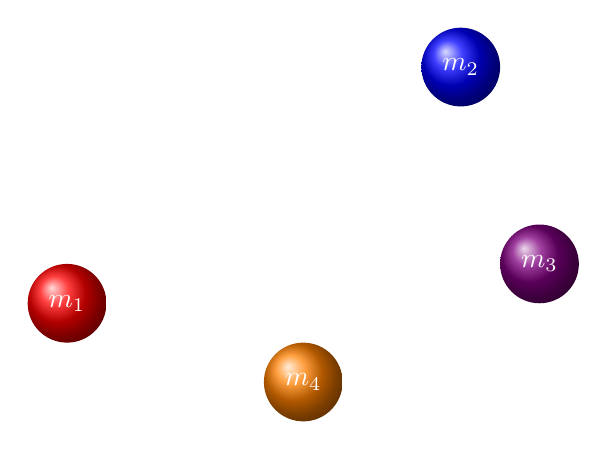
\begin{tikzpicture}
    \shade[ball color=red] circle (.5) node[white]{$m_1$};
    \shade[ball color=blue] (5,3) circle (.5) node[white]{$m_2$};
    \shade[ball color=violet] (6,.5) circle (.5) node[white]{$m_3$};
    \shade[ball color=orange] (3,-1) circle (.5) node[white]{$m_4$};
  \end{tikzpicture}
\end{figure}







%\chapter{Orbital Mechanics}
\section{Orbital Mechanics}
We turn our attention to applying the law of universal gravitation to the
orbital motion of planets and stars in our solar system. To start, two
properties of gravity are crucial to understanding of orbital mechanics:
\begin{enumerate}
\item Gravity is a \emph{conservative force}, as we have seen in
  Chapter~\ref{chapter:energy}, in that the positive work done by gravity
  converts gravitational potential energy $U_g$ into kinetic energy $K$,
  and conversely, negative work by gravity converts $K$ into $U_g$. Therefore
  the total mechanical energy of objects under gravity is constant.

\item Gravity is a \emph{central force}, in that the direction of the
  gravitational force $\bm F_g$ is always in the $-\hat{\bm r}$ direction, as
  shown in Fig.~\ref{central-force}. Therefore
  $\bm r\times\bm F=\bm\tau_g=\bm 0$. Gravity doesn't generate any torque
  about the sun, and angular momentum $\bm L$ is constant.
\end{enumerate}
\begin{figure}[!ht]
  \centering
  \begin{tikzpicture}[scale=1.2]
    \draw[vector,blue] (0,0)--(2,3) node[midway,left]{$\bm r$};
    %\draw[vector] (0,0)--(2,3) node[midway,left]{$\bm r$};
    \begin{scope}[rotate around={-33.7:(2.03,3)}]
      \draw[vector,red](2.03,3)--(2.03,1.5) node[midway,below right]{$\bm F_g$};
    \end{scope}
    \draw[vector] (2,3)--(3,2.8) node[right]{$\bm v$};
    \fill circle(.12) node[right=4]{Sun};
    \fill (2,3) circle (.07) node[left=4]{Planet};
  \end{tikzpicture}
  \caption{A central force such as gravity do not generate a torque (moment).}
  \label{central-force}
\end{figure}
These properties are true regardless of the shape of the orbit, and even
for objects that are not in orbit at all (e.g.\ an asteroid slingshotting
around the sun). In \emph{Treatise of the System of the World}, the third book
in \emph{Principia}, Newton presented a thought experiment, shown in
Fig.~\ref{fig:thought-experiment}. A cannonball is shot parallel to the surface
of Earth with some initial velocity $\bm v$.
\begin{figure}[ht]
  \centering
  \begin{subfigure}{.4\textwidth}
    \centering
    \begin{tikzpicture}
      \node at (0,0) {\pic{.45}{universalGravitation/earth-1200px}};
      \fill[red] (0,1.7) circle (.05);
      \draw[function,->] (0,1.7) arc (90:30:1 and 1.45);
      \draw[dashed,gray,thick] circle (1.7);
    \end{tikzpicture}
    \caption{At a low initial velocity, the object falls onto the planet
      after travelling only a short distance}
  \end{subfigure}
  \hspace{.3in}
  \begin{subfigure}{.4\textwidth}
    \centering
    \begin{tikzpicture}
      \node at (0,0) {\pic{.45}{universalGravitation/earth-1200px}};
      \fill[red] (0,1.7) circle (.05);
      \draw[function,->] (0,1.7) arc (90:-50:1.5 and 1.5);
      \draw[dashed,gray,thick] circle (1.7);
    \end{tikzpicture}
    \caption{With a higher initial velocity, the object travels a longer
      distance but eventually, it still falls back to the surface}
  \end{subfigure}
  
  \begin{subfigure}{.4\textwidth}
    \centering
    \begin{tikzpicture}
      \node at (0,0) {\pic{.45}{universalGravitation/earth-1200px}};
      \fill[red] (0,1.7) circle (.05);
      \draw[function,->] (0,1.7) arc (90:-270:1.7);
    \end{tikzpicture}
    \caption{At ``orbital velocity'', the object stays on a perfectly circular
      path around the planet}% without falling}
    \label{fig:in-orbit}
  \end{subfigure}
  \hspace{.3in}
  \begin{subfigure}{.4\textwidth}
    \centering
    \begin{tikzpicture}
      \node at (0,0) {\pic{.45}{universalGravitation/earth-1200px}};
      \fill[red] (0,1.7) circle (.05);
      \draw[dashed,gray,thick] circle (1.7);
      \draw[function,->,domain=0:2.2] plot(\x,{-.3*\x*\x+1.7});
    \end{tikzpicture}
    \caption{At escape velocity or higher, the object escapes the gravitational
      pull of the planet}
    \label{fig:escape-from-orbit}
  \end{subfigure}
  \caption{Newton's thought experiment}
  \label{fig:thought-experiment}
\end{figure}
We want to answer the questions:
\begin{enumerate}
\item How fast does the cannonball have to travel before it goes around Earth
  without falling? (i.e.\ goes into orbit)
\item How fast does the cannonball have to travel before it never comes back?
\end{enumerate}



\section{Orbital Speed}
\label{sec:orbital-speed}
The example shown in Fig.~\ref{fig:in-orbit} (``fast enough that it doesn't
fall down'') is that of an object moving in circular motion around the planet.
If we assume that a small mass $m$ is in a circular orbit around a much larger
mass $M$, we can further assume that $M$ is stationary. The distance $r$
between the masses is also the orbital radius of that circular motion, and the
centre of $M$ is also the centre of the circular motion. The required centripetal
force is supplied by the gravitational force. Since there are no other forces,
the object moves in uniform circular motion with a constant speed
$v_\text{orbit}$, called the \textbf{orbital speed}, and the velocity vector
$\bm v_\text{orbit}$---which is tangent to the cicular path--- is called
the \textbf{orbital velocity}. This is shown graphically in
Fig.~\ref{fig:orbital-velocity}.
\begin{figure}[ht]
  \centering
  \begin{tikzpicture}[scale=.8]
    \node at (0,0) {\pic{.12}{universalGravitation/earth-1200px}};
    \draw[function,->] (0,3) arc (90:-270:3);
    \begin{scope}[rotate=50]
      \draw[thick] (0,0)--+(0,-.8);
      \draw[very thick,<->] (0,-.5)--(3,-.5) node[midway,fill=white]{$r$};
      \fill circle (.05) node[above]{$M$};
      \draw[vector,violet] (3,0)--+(0,-2) node[right]{$\bm v_\text{orbit}$};
      \draw[mass] (3,0) circle (.07) node[above]{$m$};
    \end{scope}
  \end{tikzpicture}
  \caption{Object travelling in a circular orbit at the orbital velocity.}
  \label{fig:orbital-velocity}
\end{figure}

Starting with the second law of motion applied to circular motion,
$\bm F_c=m\bm a_c$, and substituting the gravitational force $F_g$ into
the expression for centripetal force:
\begin{equation}
  F_g=ma_c\quad\longrightarrow\quad \frac{GMm}{r^2}=\frac{mv^2}r
\end{equation}
cancelling the $r$ and $m$ terms on both sides of the equation, we can solve
for the expression for orbital speed, which does not depend on the mass $m$
of the object in orbit:
\begin{equation}
  \boxed{v_\text{orbit}=\sqrt{\frac{GM}r}}
\end{equation}
Note that this equation is only applicable for perfectly circular orbits. Like
all uniform circular motion, the direction of $\bm v_\text{orbit}$ is tangent
to the circular path.



\section{Escape Speed}
The case from Fig.~\ref{fig:escape-from-orbit} is that of an object leaving
orbit, and escaping from the gravitational pull of the planet. For this to
happen, the object must have an minimum velocity such that when all of its
kinetic energy at launch is converted into gravitational potential energy,
the object would be infinitely far away from the planet. This minimum speed
is called the \textbf{escape speed} $v_\text{esc}$.
%An object can leave the surface of Earth at any speed. But when all the
%kinetic energy of that object is converted to gravitational potential energy,
%it will return back to the surface of the earth. There is, however, a
%\emph{minimum} velocity at which the object \emph{would not} fall back to
%Earth.

To find the expression for escape speed, we make the following assumptions:
\begin{itemize}
\item The mass of ($m$) of the object being launched from the planet ($M$) is
  constant
\item Gravitational force is the only force acting on $m$, and that there is
  no friction, drag, or thrust from the rocket's engines
\end{itemize}
These assumptions are, of course, very unrealistic if you want to launch a
rocket from Earth: the mass of a rocket launched from Earth will change very
rapidly, and as the rocket travels into space at supersonic speeds, the drag
that it encounters is very high. However, these assumptions would be more
applicable to someone ``tossing'' an object away from a planet that has no
atmosphere. Under these assumptions, the calculation for escape speed is a
simple exercise in conservation of energy:
\begin{equation}
  K_\text{launch} + U_\text{launch} = K_\infty + U_\infty
\end{equation}
On the left hand side of the equation, the initial gravitational potential
energy at the surface is:
\begin{equation}
  U_\text{launch}=-\frac{GMm}{r_i}
\end{equation}
where $r_i$ is the object's initial distance from the centre of the
planet/star\footnote{The object does not have to be launched from the
surface.}. The kinetic energy at launch is:
\begin{equation}
  K_\text{launch}=\frac12mv_\text{esc}^2
\end{equation}
the speed $v_\text{esc}$ at launch is the escape speed that we are seeking. On
the right hand side of the equation, the final gravitational potential energy
is at $r_f=\infty$, where $U_\infty=0$. At this point, the object has already
\emph{escaped} the gravitational pull of the planet/star $M$. At this point, it
no longer matters whether the object is in motion or not, therefore the minimum
required kinetic energy at $r=\infty$ is $K_\infty=0$. Setting the right-hand
side to zero, and equating $K_\text{launch}$ to equal to $-U_\text{launch}$, we
get:
%\item The work against gravity converts kinetic energy into gravitational
%  potential energy.
%\item If you start with \emph{more} kinetic energy than required to do all
%  the work, then the object has
%  planet.
%\end{itemize}
\begin{equation}
  \frac12mv_\text{esc}^2=\frac{GMm}{r_i}
\end{equation}
We can then solve for the escape speed:
\begin{equation}
  \boxed{
    v_\text{esc}=\sqrt{\frac{2GM}{r_i}}
  }
  \label{eq:escape-speed}
\end{equation}
There is a simple relationship between orbital speed and escape speed:
\begin{equation}
  v_\text{esc}=\sqrt2v_\text{orbit}
\end{equation}

\begin{example}
  Determine the escape speed for a \SI{1.60e4}{\kilo\gram} rocket leaving the
  surface of Earth.
    
  \vspace{.2in}
  \textbf{Solution:} All we have to do is to substitute the correct values into
  Eq.~\ref{eq:escape-speed}. The mass of Earth is $M=\SI{5.791e24}{\kilo\gram}$,
  and the rocket launched from Earth's surface, so $r_i=r_E=\SI{6.371e6}\metre$:
  \begin{equation*}
    v_\text{esc}
    =\sqrt{\frac{2GM}{r_i}}
    =\sqrt{\frac{2\times \num{6.67e-11}\times\num{5.792e24}}{\num{6.371e6}}}
    =\SI{1.12e4}{\metre\per\second}
  \end{equation*}
  This means that the object leaves the surface at more than
  \SI{11}{\kilo\metre\per\second}. Consider that commercial airliners fly at
  about \SI{13}{\kilo\metre} in altitude, the rocket will reach that height in
  just over 1 second. The rocket's mass, although is given to you, is not
  required in solving the problem.
\end{example}

The equation for the escape speed is based on:
\begin{itemize}
\item The object have a \emph{constant} mass
\item All the work is done by gravitational force
\end{itemize}
Neither of which apply to the case for a rocket going into space. In reality, a
rocket will reach hypersonic (about Mach 5) speeds at launch, and therefore
have an enormous amount of drag force acting on it. Additionally, the mass of a
rocket is mostly in its fuel, while the mass of the structure, engines, and
payload comprises of a very small percentage of the weight at launch.

The equation for escape speed is more suited if an object is \emph{catapulted}
from a planet or moon that does not have an atmoshere. Nevertheless,
Eq.~\ref{eq:escape-speed} gives us an approximation to the speed that is needed
to escape the gravitational pull of a planet.

It is also important to note that the object can escape from the \emph{surface}
or the planet, or it can escape from \emph{orbit}.
In Fig.~\ref{fig:two-escapes}, both objects have the same escape velocity.
\begin{figure}[ht]
  \centering
  \begin{subfigure}{.4\linewidth}
    \centering
    \begin{tikzpicture}[scale=1.8]
      \node at (0,0) {\pic{.15}{universalGravitation/earth-1200px}};
      \draw[thick] circle (.25) node[below]{$M$};
      \draw[thick,dashed] circle (1);
      \draw[mass] (0,1) circle (.05);
      \draw[mass] (2,0) circle (.05);
      \draw[thick,<->] (0,0)--(0,1) node[midway,right=0]{$r$};
      \draw[vector,red] (0,1) to[out=0,in=135] (2,0);
    \end{tikzpicture}
  \end{subfigure}
  \begin{subfigure}{.4\linewidth}
    \centering
    \begin{tikzpicture}[scale=1.8]
      \node at (0,0) {\pic{.61}{universalGravitation/earth-1200px}};
      \draw[thick] circle (1) node[below]{$M$};
      \draw[mass] (0,1) circle (.05);
      \draw[mass] (2,0) circle (.05);
      \draw[thick,<->] (0,0)--(0,1) node[midway,right]{$r$};
      \draw[vector,red] (0,1) to[out=0,in=135] (2,0);
    \end{tikzpicture}
  \end{subfigure}
  \caption{Escape velocity only depends on $M$ and $r$}
  \label{fig:two-escapes}
\end{figure}
The difference is that the object in orbit (left) already has orbital speed
$v_\text{orbit}$, so escaping from that orbit requires only an additional
speed of
\begin{equation}
  \Delta v=v_\text{esc}-v_\text{orbit}=(\sqrt2-1)v_\text{orbit}
\end{equation}



\section{Orbital Energies}
We can obtain the \textbf{orbital kinetic energy} in a perfectly circular orbit
by using the orbital speed in our expression of kinetic energy, for when a small
object is orbiting around a much larger mass:
\begin{equation}
  K_\text{orbit}=\frac12mv_\text{orbit}^2=\frac12m
  \left(\sqrt{\frac{GM}r}\right)^2=\boxed{\frac{GMm}{2r}}
\end{equation}
We already have an expression for gravitational potential energy:
\begin{equation}
    U_g=-\frac{GMm}r=-2K_\text{orbit}
\end{equation}
The ratio between gravitational potential energy and kinetic energy
($U_g=-2K_\text{orbit}$) is not unique to gravity. An electron that ``orbits''
around a much heavier nucleus also has the same ratio between \emph{electric}
potential energy and kinetic enery.

The \textbf{total orbital energy} is the sum of $K$ and $U_g$:
\begin{equation}
  E_T=K_\text{orbit}+U_g=-\frac{GMm}{2r}=-K_\text{orbit}
\end{equation}
\textbf{Binding energy}, or \textbf{escape energy} is the energy to remove the
object from the planet's orbit, is the energy make
\begin{equation}
  E_b=-E_T=K_\text{orbit}
\end{equation}



\section{Binary Star Systems}
It is true that a majority of orbital motions we observer in the our solar
system are of type described in Section~\ref{sec:orbital-speed}, where a small
mass orbits around a much larger mass. This may be a moon or satellite, or even
space debris, orbiting around a planet, or it could be a planet, or comet, or
asteroids orbiting the sun. However, there are situations where two objects
of comparable masses orbit each other. In Fig.~\ref{fig:binary1}, two stars of
mass $m_1\approx m_2$ are in circular orbit around each other. Both stars orbit
a common orbital centre which is the centre of mass of the binary system.
Gravitational force still provides the centripetal force.
\begin{figure}[ht]
  \centering
  \begin{tikzpicture}[scale=.4]
    \fill circle (.2) node[left]{cm};
    \draw[dashed] circle (4);
    \draw[dashed] circle (8);
    %\draw[axes,rotate=30] (0,0)--(0,8) node[above]{$r_1$};
    %\draw[axes,rotate=-110] (0,0)--(4,0) node[below]{$r_2$};
    \draw[vector,blue] (-8,0)--+(0,3) node[above]{$\bm v_1$};
    \draw[vector,red] (4,0)--+(0,-6) node[below]{$\bm v_2$};
    \draw[vector,blue] (-8,0)--+(1.5,0) node[above]{$\bm F_g$};
    \draw[vector,red] (4,0)--+(-3,0) node[above]{$\bm F_g$};
    \node at (-8,0) {\pic{.03}{universalGravitation/blue-star1}};
    \node at (4,0) {\pic{.06}{universalGravitation/orange-star1}};
    \draw[|<->|] (-8,-2.5)--+(8,0) node[midway,fill=white]{$r_1$};
    \draw[<->] (0,-2.5)--+(4,0) node[midway,fill=white]{$r_2$};
  \end{tikzpicture}
  \caption{Two stars of comparable masses in circular orbital motion about
    their centre of mass}
  \label{fig:binary1}
\end{figure}    

\begin{example}[Binary Star System]
  Two stars of mass $m_1$ and $m_2=2m_1$ orbit each other, i.e.\ they orbit
  around their centre of mass. From Chapter~\ref{chapter:cm}, we know that the
  orbital distances are related by $r_1=2r_2$. To find the orbital speed of
  $m_1$, Setting the gravitational force to be the centripetal force:
  \begin{equation*}
    F_c=ma_c\quad\rightarrow\quad \frac{Gm_1m_2}{(r_1+r_2)^2}=\frac{m_1v_1^2}{r_1}
  \end{equation*}
  Unlike the case in Section~\ref{sec:orbital-speed}, the orbital radius $r_1$
  is \emph{not} the distance between the stars, which is $r_1+r_2$. Setting
  $m_2=2m_1$ and $r_2=r_1/2$, the equation becomes:
  \begin{equation*}
    \frac{Gm_1(2m_1)}{[r_1+(r_1/2)]^2}=\frac{m_1v_1^2}{r_1}
    \quad\rightarrow\quad
    \frac{8Gm_1^2}{9r_1^2}=\frac{m_1v_1^2}{r_1}
  \end{equation*}
  Cancelling the $m_1$ and $r_1$ terms on both sides, just as we did in
  Section~\ref{sec:orbital-speed}, we find the orbital speed for $m_1$ is:
  \begin{equation*}
    v_1=\sqrt{\frac{8Gm_1}{9r_1}}
  \end{equation*}
  For the orbital speed of $m_2$, we repeat the same procedure as above:
  \begin{equation*}
    F_c=ma_c
    \quad\rightarrow\quad
    \frac{Gm_1m_2}{(r_1+r_2)^2}=\frac{m_2v_2^2}{r_2}
    \quad\rightarrow\quad
    \frac{4Gm_1m_2}{9r_1^2}=\frac{2m_2v_2^2}{r_1}
  \end{equation*}
  Cancelling the $m_2$ and $r_1$ terms, we find the orbital speed for $m_2$,
  which is half that of for $m_1$:
  \begin{equation*}
    v_2=\sqrt{\frac{2Gm_1}{9r_1}}=\frac12v_1
  \end{equation*}
  $m_2$ orbits at half the radius and halt the speed. This means that both
  stars have the same orbital period. This should make sense if the orbits are
  to remain stable.
\end{example}




\section{Elliptical Orbits}
As shown in Fig.~\ref{fig:circular-elliptical-parabolic-hyperbolic},
depending on the magnitude of $\bm v$ at $P$:
\begin{figure}[ht]
  \centering
  \begin{tikzpicture}
    \node at (0,0) {\pic{.28}{universalGravitation/earth-1200px}};
    \draw[vector,red] (0,4) arc (90:-250:4);
    \draw[vector,violet,domain={0:4},dash dot] plot(\x,-.1*\x*\x+4);
    %node[right]{$v_\text{esc}$ (parabola)};
    \draw[very thick,blue,dotted] (0,.5) ellipse (3.2 and 3.5);
    \draw[very thick,orange,dashed] (0,-.5) ellipse (4.2 and 4.5);
    \draw[mass] (0,4) circle (.08) node[above]{$P$};
    \draw[vector] (0,4)--(1.5,4) node[above]{$\bm v$};
    \fill (0,-3) circle (.08) node[below]{$P'$};
    \fill (0,-5) circle (.08) node[below]{$P''$};
    \node[above,blue] at (0,-3) {\scriptsize Elliptical};
    \node[above,magenta] at (0,-4) {\scriptsize Circular};
    \node[above,orange] at (0,-5) {\scriptsize Elliptical};
    \draw[thick,|<->] (0,0)--(0,4) node[pos=.6,right]{$r$};
  \end{tikzpicture}
  \caption{Different orbital paths}
  \label{fig:circular-elliptical-parabolic-hyperbolic}
\end{figure}
\begin{itemize}[leftmargin=18pt]
\item{\color{magenta}If the object moves at orbital velocity, i.e.\
  $v=v_\text{orbit}$, it will orbit around the planet in uniform circular
  motion. The path is perfectly circular, and the speed is constant.}
  
\item{\color{violet}If the object is at escape velocity, $v=v_\text{esc}$, it
  will leave the planet's gravitational pull in a parabolic path.}
  
\item{\color{green!80!black}If the object is faster than escape velocity, i.e.\
    $v>v_\text{esc}$, it will leave the planet's gravitational pull in a
  hyperbolic path.}
  
\item{\color{orange} If the object is moving faster than the orbital speed, but
  not faster enough for escape speed, i.e.\ $v_\text{orb}<v<v_\text{esc}$, the
  object would be too fast to maintain a circular path, and therefore gain
  altitude, arriving at point $P'$ on the other side of the planet, which is
  the furthest away from the centre. the resulting path is elliptical.}
  
\item{\color{blue} If the object is moving slower than the orbital speed, i.e.\
  $v<v_\text{orb}$, the object would lose altitude, arriving at point $P''$ on
  the other side of the planet, which is the closest away from the centre. The
  resulting path is also elliptical. The object does not necessarily crash; that
  will depend on what the actual speed is.}
\end{itemize}



\section{Kepler's Laws of Planetary Motion}

Johannes Kepler\footnote{1571--1630. German mathematician, astronomer and
  astrologer.} formulated his \textbf{laws of planetary motion}
between 1609 to 1619, by carefully interpreting the empirical planetary motion
data from his teacher, Tycho Brahe.\footnote{1546--1601. Danish nobleman and
  astronomer.} It is an improvement over the heliocentric
theory of Nicolaus Copernicus\footnote{1473--1543. German mathematician,
  astronomer and Catholic canon.}. It should be noted that the complete
mathematical understanding was missing until Issac Newton\footnote{1642--1726.
  English mathematician, physicist, astronomer, theologian, and author.}
derived each law as using his laws of motion. Here, we seek to obtain
each law, as we consider the orbit of a small planet in the gravitational field
of a much more massive star. Expressed in modern language:
\begin{enumerate}
\item\textbf{Law of ellipses:} The orbit of a planet is an ellipse with the
  Sun at one of the two foci.
\item\textbf{Law of equal areas:} A line segment joining a planet and the Sun
  sweeps out equal areas during equal intervals of time
\item \textbf{Law of periods:} The square of the orbital period of a planet
  is proportional to the cube of the semi-major axis of its orbit.
\end{enumerate}
For the purpose of the analysis, we assume that the Sun's mass $M_\odot$
is very large compared to any other object in the solar system (planets,
comets, asteroids, etc.), and its motion is essentially unaffected by the
gravity from them.



\subsection{Law of Ellipses}
Kepler's first law, called the \textbf{law of ellipses}, is more difficult to
proof. In order to proof the
law, we must show that all orbital motion must agree with the equations of an
ellipse. An ellipse is shown in Fig.~\ref{ellipse1} with the origin of the
coordinate system located at one of the two foci.
\begin{figure}[!ht]
  \centering
  \begin{tikzpicture}[scale=.8]
    \def\a{4}       % semi-major axis
    \def\b{3.25}    % semi-minor axis
    \def\angle{150} % angle
    \draw[very thick] ellipse ({\a} and {\b});% Draw the ellipse
    \draw[axes] ({sqrt(\a*\a-\b*\b)},-3.5)--({sqrt(\a*\a-\b*\b)},3.5)
    node[above]{$y$};
    \draw[axes] (-\a-.2,0)--(\a+.5,0) node[right]{$x$};
    \begin{scope}[rotate around={\angle:({sqrt(\a*\a-\b*\b)},0)}]
      \draw[red,thick]({sqrt(\a*\a-\b*\b)},0)--(7.66,0) node[pos=.7,below]{$r$};
      \fill[red] (7.66,0) circle (.04);
    \end{scope}
    \begin{scope}[rotate around={-91.1:({-sqrt(\a*\a-\b*\b)},0)}]
      \draw[red,thick]({-sqrt(\a*\a-\b*\b)},0)--(-5,0) node[midway,left]{$r'$};
    \end{scope}
    \draw[axes] ({sqrt(\a*\a-\b*\b)+.5},0) arc (0:\angle:.5)
    node[pos=.4,above]{$\theta$};
    %\draw[<->]({sqrt(\a*\a-\b*\b)-.2},0)--({sqrt(\a*\a-\b*\b)-.2},-2.65)
    %node[midway,left]{\tiny$r_0$};
    \fill ({sqrt(\a*\a-\b*\b)},0) circle (.05) node[below]{$f_1$};
    \fill ({-sqrt(\a*\a-\b*\b)},0) circle (.05) node[below]{$f_2$};
    \draw[very thick,blue] (0,0)--(\a,0) node[midway,below]{$a$};
    \draw[very thick,blue] (0,0)--(-\a,0) node[midway,below]{$a$};
    \draw[very thick,orange] (0,0)--(0,\b) node[midway,right]{$b$};
    \draw[very thick,orange] (0,0)--(0,-\b) node[midway,right]{$b$};
    \fill circle (.05) node[below right]{$C$};
  \end{tikzpicture}
  \caption{A basic ellipse with the origin of the coordinate system placed at
    one of the focus.}
  \label{ellipse1}
\end{figure}

The longer dimension from the origin is the \textbf{semi-major axis} $a$, while
the shorter dimension is the \textbf{semi-minor axis} $b$. The two lengths are
related by the parameter $e$, the \textbf{eccentricity} of the ellipse:
\begin{equation}
  b^2=a^2(1-e^2)\quad\text{where}\quad 0\leq e < 1
\end{equation}
When the eccentricity of a planet's orbit is zero, the orbit is perfectly
circular, and $a=b=r$. As $e\rightarrow 1$, the orbit is stretched out into
more elongated elliptical trajectories. At $e=1$, the shape becomes a parabola,
and is no longer an ellipse.

The area $A$ of an ellipse is given by the semi-major and semi-minor axes:
\begin{equation}
  A=\pi ab=\pi a^2\sqrt{1-e^2}
  \label{A2}
\end{equation}
When the origin of the coordinate system placed one of the two foci, an ellipse
can be expressed using polar coordinates:
\begin{equation}
  r=\frac{a(1-e^2)}{1+e\cos\theta}
  \label{ellipse-eq}
\end{equation}

As shown in Fig.~\ref{eorbit}, there are two components of velocity when a
planet orbits a star:
\begin{figure}[!ht]
  \centering
  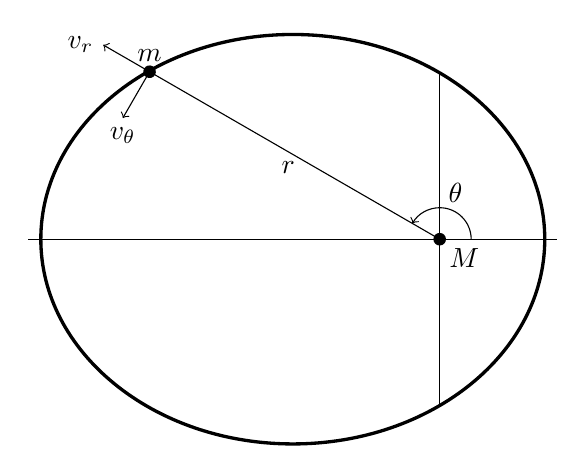
\begin{tikzpicture}[scale=.8]
    \def\a{4}       % semi-major axis
    \def\b{3.25}    % semi-minor axis
    \def\angle{150} % angle
    \draw[very thick] ellipse ({\a} and {\b});% Draw the ellipse
    \draw ({sqrt(\a*\a-\b*\b)},-2.65)--({sqrt(\a*\a-\b*\b)},2.65);
    \draw (-\a-.2,0)--(\a+.2,0);
    \fill ({sqrt(\a*\a-\b*\b)},0) circle(.1) node[below right]{$M$};
    \begin{scope}[rotate around={\angle:({sqrt(\a*\a-\b*\b)},0)}]
      \draw[->]({sqrt(\a*\a-\b*\b)},0)--(8.5,0)
      node[pos=.45,below]{$\bm r$} node[left]{$\bm v_r$};
      \draw[->](7.65,0)--(7.65,.85) node[below]{$\bm v_\theta$};
      \fill (7.65,0) circle(.1) node[above]{$m$};
    \end{scope}
    \draw[->]({sqrt(\a*\a-\b*\b)+.5},0) arc (0:\angle:.5)
    node[pos=.4,above]{$\theta$};
  \end{tikzpicture}
  \caption{Elliptical orbit of a small mass $m$ around a large mass $M$.}
  \label{eorbit}
\end{figure}
\begin{itemize}
\item\textbf{Angular velocity} $\bm v_\theta$. The presence of
  $\bm v_\theta$ means that there is a centripetal acceleration $a_c$ toward
  $M$. The direction of the acceleration is perpendicular to the direction of
  $\bm v_\theta$, and toward the sun:
  \begin{equation}
    a_c=-r\omega^2\hat{\bm r}
  \end{equation}
\item\textbf{Radial velocity} $\bm v_r$. If this velocity is non-zero and
  changes with time (which is the case for elliptical orbits but not for
  circular orbits), then there is an acceleration $a_r$, also in the radial
  direction:
  \begin{equation}
    a_r=\diff{v_r}t\hat{\bm r}=\diff[2]rt\hat{\bm r}
  \end{equation}
\end{itemize}
Both components of acceleration are due entirely to gravitational force.
Applying second law of motion, and dividing all sides by the mass of the planet
$m$, we arrive at a differential equation:
\begin{equation}
  \diff[2]rt-r\omega^2=-\frac{GM}{r^2}
  \label{ode1}
\end{equation}
In this equation, the ($+$) direction is radially outward from $M$. In the
circular motion case, where $\ddot r=0$, we are left with only the centripetal
acceleration $a_c=r\omega^2$ which is expected in uniform circular motion. The
differential equation, in its present form, is difficult to solve. Moreover,
the equation that for an ellipse (Eq.~\ref{ellipse-eq}) depends on $\theta$ but
not on $t$. However, the differential equation is easier to solve by making a
variable substitution\footnote{this variable may not be immediately obvious
  without some experience with solving ODEs}, by introducing a new variable $u$
which is the reciprocal of $r$:
\begin{equation}
  u=\frac1r
\end{equation}
We can then use the fact that angular momentum $L$ is constant to relate
derivatives in time $t$ to derivatives in angle $\theta$:
\begin{equation}
  L=mr^2\omega=mr^2\diff{\theta}t=\frac m{u^2}\diff{\theta}t
  \quad\longrightarrow\quad
  \diff{\theta}t=\frac{Lu^2}m
\end{equation}
The derivative $\dot r$ can now be expressed in terms of derivatives of
$\theta$ instead of time $t$:
\begin{equation}
  \diff rt =\diff*{\left(\frac1u\right)}t
  =-\frac1{u^2}\diff ut=-\frac1{u^2}\diff u\theta\diff{\theta}t
  = -\frac1{u^2}\diff u\theta \frac{Lu^2}m
  = -\frac Lm\diff u\theta
\end{equation}
Repeating the same process for the second derivative $\ddot r$, we have
\begin{equation}
  \diff[2] rt = \diff*{\left(-\frac Lm\diff u\theta\right)}t
  = -\frac Lm\diff*{\left(\diff u\theta\right)}\theta \\
  = -\left(\frac{L^2u^2}{m^2}\right)\diff[2]u\theta
\end{equation}
With this identity in hand, our original differential equation
(Eq.~\ref{ode1}) becomes
\begin{equation}
  -\left(\frac{L^2u^2}{m^2}\right)\diff[2]u\theta-\left(\frac Lm\right)^2u^3
  = -GMu^2
\end{equation}
which can be simplified to:
\begin{equation}
  \diff[2]u\theta + u = \frac{GMm^2}{L^2}
  \label{newdiff}
\end{equation}
Anyone experienced with calculus can recognize that Eq.\ \ref{newdiff} is a
\emph{second-order ordinary differential equation with constant coefficients
  and a constant forcing function}. The solution to this type of equation is in
the form
\begin{equation} 
  u =B\cos\theta + \frac{GMm^2}{L^2}
\end{equation}
where the coefficient $B$ is determined by the total energy and total angular
momentum (both are constants) of the planets. Solving for $r=1/u$, we have
\begin{equation}
  r(\theta)=\frac1u = \frac1{B\cos\theta+ \dfrac{GMm^2}{L^2}}
  =\left(\dfrac{L^2}{GMm^2}\right)\frac1{1+e\cos\theta}
\end{equation}
where $e$ is a constant:
\begin{equation}
  e=\dfrac{BL^2}{GMm^2}
\end{equation}
It should become obvious that this $e$ is, in fact, the eccentricity of the
elliptical orbit previously mentioned. If a planet, or any celestial object
has too much total energy when it enters the gravitational field of the sun,
then $e>1$, and the object will not return. From this form of $r$, it is clear
that the maximum and a minimum values of $r$ represent the \emph{aphelion} and
\emph{perihelion} of an ellipse (points of furthest and closest distance to the
focus):
\begin{equation}
  r_\text{max}=\left(\frac{L^2}{GMm^2}\right)\frac1{1-e}
  \quad\quad
  r_\text{min}=\left(\frac{L^2}{GMm^2}\right)\frac1{1+e}
\end{equation}
This the semi-major axis $r$ is the average of the two values:
\begin{equation}
  a=\dfrac12\left(r_\text{min} + r_\text{max}\right)=
  \left(\frac{L^2}{GMm^2}\right)\frac1{1-e^2}
  \label{semimajor}
\end{equation}
More importantly, Eq.\ \ref{semimajor} allows us to relate the eccentricity
$e$ and the semi-major axis $a$ to the numerator in the $r$ expression:
\begin{equation}
  a(1-e^2)=\frac{L^2}{GMm^2}
  \label{eq:numerator}
\end{equation}
We see that the orbit is given by an ellipse as Kepler found from Brahe's data.
Moreover, since $r_\text{min}$ and $r_\text{max}$ are distances from the Sun, we
see that the Sun is at one focus of the orbit. Thus, we have derived Kepler's
first law.


\subsection{Law of Equal Area}

The second law of planetary motion, called the \textbf{law of equal areas},
states (in modern terms) that line segment joining a planet and the Sun sweeps
out equal areas during equal intervals of time (Fig.~\ref{kep2}). The second
law of planetary motion is the easiest to proof using concepts in rotational
motion.
\begin{figure}[!ht]
  \centering
    \pic{.4}{keplers-laws/201532-132212364-3243-planet}
    \caption{The Earth sweeps out the same shaded area (purple) over the
      same amount of time regardless of where it is in its orbit.}
    \label{kep2}
\end{figure}

To begin, recognize that for a planet with a velocity vector $\bm v$ that is
not co-linear with the displacement vector $\bm r$ will sweep out an
infinitesimal area $\dl{\bm A}$ (Fig.~\ref{fig:dA})
\begin{figure}[ht]
  \centering
  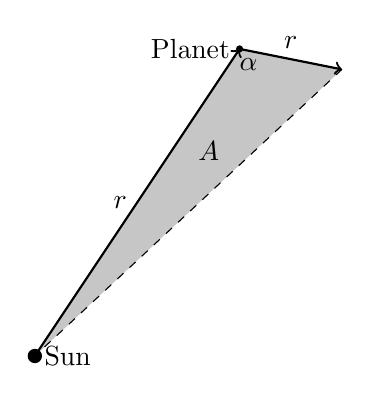
\begin{tikzpicture}[scale=1.3]
    \fill[gray!45](0,0)--(2,3)--(3,2.8)--cycle;
    \node at (1.7,2) {$\dl{\bm A}$};
    \draw[->,thick] (0,0)--(2,3)
    node[midway,left]{$\bm r$} node[pos=.95,right]{$\alpha$};
    \draw[->,thick] (2,3)--(3,2.8) node[midway,above]{$\dl{\bm r}$};
    \draw[dashed] (3,2.8)--(0,0);
    \fill circle (.07) node[right]{Sun};
    \fill (2,3) circle (.035) node[left]{Planet};
  \end{tikzpicture}
  \caption{Infinitesimal area $\dl{\bm A}$ swept by a planet as it moves
    $\dl{\bm r}$ in orbit.}
  \label{fig:dA}
\end{figure}
as it moves in orbit by an infinitesimal amount $\dl{\bm r}$, which can be
computed by the area of the triangle:
\begin{equation}
  \dl A=\frac12r\dl r\sin\alpha
\end{equation}
or in vector form:
\begin{equation}
  \dl{\bm A}=\frac12\bm r\times\dl{\bm r}
\end{equation}
The direction of $\dl{\bm A}$, in this case, points into the page.\footnote{The
  direction of the vector is not important in the calculation, but is only used
  to formalize the vector operations.} The time derivative of the area is
called the \textbf{areal velocity}, which literally means how quickly the area
is changing:
\begin{equation}
  \diff{\bm A}t
  =\frac12\bm r\times\diff{\bm r}t
  =\frac12\bm r\times\bm v
\end{equation}
We can express $\bm r\times\bm v$ in terms of angular momentum. Since
angular momentum is defined as $\bm L=m(\bm r\times\bm v)\;\rightarrow\;
\bm r\times\bm v=\bm L/m$. Since gravity is a central force, angular
momentum is a constant, i.e:
\begin{equation}
  \boxed{\diff{\bm A}t=\frac12(\bm r\times\bm v)=\frac{\bm L}{2m}=
    \text{constant}
  }
  \label{constant}
\end{equation}
as predicted by Kepler's second law. The rate that a planet sweeps out the area
in orbit is its angular momentum around the sun, divided by twice its mass. It
is constant regardless of its location relative to the sun.




\subsection{Law of Periods}
\begin{figure}[!ht]
  \centering
  \begin{tikzpicture}[xscale=1.5]
    \draw[very thin,gray!40] grid (7.5,7.5);
    \draw[axes] (0,0)--(7.5,0) node[right]{$T^2$ ($\text{yr}^2$)};
    \draw[axes] (0,0)--(0,7.5) node[above]{$a^3$ ($\text{AU}^3$)};
    \foreach \x in {0,...,6}{
      \draw[thick] (\x+1,0)--(\x+1,-.2) node[below]{$10^{\x}$};
      \draw[thick] (0,\x+1)--(-.2,\x+1) node[left]{$10^{\x}$};
    }
    \draw[thick] (0,0)--(7,7);
    \node at (.22,.22) {\pic{.008}{universalGravitation/mercury}};
    \node at (.54,.54) {\pic{.008}{universalGravitation/venus}};
    \node at (1,1) {\pic{.008}{universalGravitation/Earth-planet}};
    \node at (1.53,1.53) {\pic{.008}{universalGravitation/mars}};
    \node at (3.15,3.15) {\pic{.06}{universalGravitation/jupiter}};
    \node at (3.93,3.93) {\pic{.09}{universalGravitation/saturn}};
    \node at (4.9,4.9) {\pic{.018}{universalGravitation/uranuscrop}};
    \node at (5.44,5.44) {\pic{.018}{universalGravitation/Neptune-planet}};
    \node at (6.08,6.08) {\pic{.01}{universalGravitation/pluto}};
  \end{tikzpicture}
  %\pic{.55}{keplers-laws/kep8}
  \caption{The orbits of all the planets in the solar system obey the third
  law of planetary motion.}
  \label{3rdlaw}
\end{figure}
In the third law, called the \textbf{law of periods}, the total area $A$ swept
by the planet through one orbital period is the areal velocity (which is
constant, as shown in Eq.\ \ref{constant}) integrated by time, from $t=0$ to
$T$, the orbital period of the planet:
\begin{equation}
  A=\int\dl A=\int_0^T\diff At\dl t=\frac L{2m}\int_0^T\dl t=\frac{LT}{2m}
  \label{A1}
\end{equation}
From proofing Kepler's first law in the previous section, we know that the
area $A$ is in the form of an ellipse, given in Eq.~\ref{A2}. Solving for
period $T$ in Eq.~\ref{A1}, then substituting the expression for area from
Eq.~\ref{A2}, and then squaring both sides, we arrive at this expression:
\begin{equation}
  T^2=\frac{m^2}{L^2}4\pi^2a^4(1-e^2)
  \label{eq:almost}
\end{equation}
Substituting Eq.~\ref{eq:numerator} into Eq.\ \ref{eq:almost} above, and after
some simple algebra, we arrive at this expression:
\begin{equation}
  \boxed{T^2=\left[\frac{4\pi^2}{GM}\right] a^3}
\end{equation}
which is Kepler's third law. Note that this law holds for all elliptical
orbits, regardless of their eccentricities.


%Johannes Kepler (1571--1630) formulated the \textbf{laws of planetary motion}
%between 1609 to 1619, by interpreting planetary motion data from his teacher,
%Tycho Brahe. It is an improvement over the heliocentric theory of Nicolaus
%Copernicus. 
%\end{enumerate}
%
%
%
%\subsection{Second Law}
%
%\begin{center}
%  \fbox{
%    \begin{minipage}{.97\textwidth}
%      \textbf{Law of Equal Areas: A line segment joining a planet and the Sun
%        sweeps out equal areas during equal intervals of time}
%    \end{minipage}
%  }
%  
%  \pic{.4}{universalGravitation/201532-132212364-3243-planet}
%\end{center}
%The second law of planetary motion is the easiest to proof, by applying the
%conservation of angular momentum $\bm L=m(\bm r\times\bm v)$ (gravity is a
%central force).
%
%
%%\begin{frame}{Kepler's Second Law: Law of Equal Areas}
%%  \begin{center}
%%    \fbox{
%%      \begin{minipage}{.9\textwidth}
%%        \textbf{A line segment joining a planet and the Sun sweeps out equal
%%          areas during equal intervals of time}
%%      \end{minipage}
%%    }
%%  \end{center}
%
%%    \begin{tikzpicture}[scale=1.3]
%%      \fill[gray!45](0,0)--(2,3)--(3,2.8)--cycle;
%%      \node at (1.7,2) {$d\bm{A}$};
%%      \draw[->,thick](0,0)--(2,3)
%%      node[midway,left]{$\bm r$} node[pos=.95,right]{$\alpha$};
%%      \draw[->,thick](2,3)--(3,2.8) node[midway,above]{$d\bm r$};
%%      \draw[dashed](3,2.8)--(0,0);
%%      \fill (0,0) circle (.07) node[right]{\tiny\text{Sun}};
%%      \fill (2,3) circle (.035) node[above]{\tiny\text{Planet}};
%%    \end{tikzpicture}
%
%%    The infinitesimal area $d\bm{A}$ swept out by an object (such as a planet)
%%    as it moves in orbit by an infinitesimal amount $d\bm r$ is given by:
%%    
%%    \eq{-.4in}{
%%      dA=\frac12rdr\sin\alpha
%%      \;\rightarrow\;
%%      d\bm{A}=\frac12\bm r\times d\bm r
%%    }
%%
%%    \vspace{-.15in}Its time derivative is called the \textbf{areal velocity}:
%%      
%%    \eq{-.15in}{
%%      \frac{d\bm{A}}{dt}
%%      =\frac12\bm r\times\frac{d\bm r}{dt}
%%      =\frac12\bm r\times\bm{v}
%%    }
%
%The rate of change of the area ($\dl A/\dl t$) swept out by a planet (called
%the \textbf{areal velocity}) is given by:
%\begin{equation}
%  \diff At=\frac L{2m}=\text{constant}
%\end{equation}
%
%The rate a planet sweeps out the area in orbit is its angular momentum around
%the sun divided by twice its mass.
%
%
%
%\subsection{First Law}
%Proofing Kepler's first law requires some understanding the ellipse. If
%the law is true, then orbital motion must agree with the equations of an
%ellipse.
%%\begin{center}
%%  \pic{1.1}{universalGravitation/elliporb}
%%\end{center}
%  
%%  \begin{itemize}
%%  \item $r' + r =2a$
%%  \item The area of the ellipse is $A=\pi ab$
%%  \item The relationship between $r$ and $\theta$ given by:
%%
%%    \eq{-.1in}{
%%        r=\frac{a(1-e^2)}{1+e\cos\theta}
%%        \quad\textnormal{\normalsize where}\quad
%%        0\leq e < 1
%%      }
%%    \item when $e=0$ it's a circle: $a=b=r$
%%    \item When $e=1$ it's no longer an ellipse
%%    \end{itemize}
%
%
%Most planets in the solar system have very small eccentricity, so their
%orbits are fairly close to being circular, but comets are much more eccentric
%%\begin{center}
%%  \pic{.65}{universalGravitation/kep5}
%%\end{center}
%\begin{table}[ht]
%  \centering
%  \begin{tabular}{l|l}
%    \rowcolor{pink}
%    \textbf{Object} & $e$ \\ \hline
%    Mercury	& \num{.206} \\
%    Venus	& \num{.0068} \\
%    Earth	& \num{.0167} \\
%    Mars	& \num{.0934} \\
%    Jupiter	& \num{.0485} \\
%    Saturn	& \num{.0556} \\
%    Uranus	& \num{.0472} \\
%    Neptune	& \num{.0086} \\
%    Pluto	& \num{.25} \\ \hline
%    Halley's Comet   & \num{.9671} \\
%    Comet Hale-Bopp  & \num{.9951} \\
%    Comet Ikeya-Seki & \num{.9999}
%  \end{tabular}
%\end{table}
%
%As $m$ orbits around $M$, there are two velocity components: \textbf{radial
%  velocity} $\bm v_r$ and \textbf{angular velocity} $\bm v_\theta$.
%\begin{center}
%  \begin{tikzpicture}[scale=.55]
%    \def\a{4} % semi-major axis
%    \def\b{3.25} % semi-minor axis
%    \def\angle{150} % angle
%    \draw ellipse ({\a} and {\b});% Draw the ellipse
%    \draw ({sqrt(\a*\a-\b*\b)},-2.65)--({sqrt(\a*\a-\b*\b)},2.65);
%    \draw (-\a-.2,0)--(\a+.2,0);
%    \fill ({sqrt(\a*\a-\b*\b)},0) circle (.1) node[below right]{$M$};
%    \begin{scope}[rotate around={\angle:({sqrt(\a*\a-\b*\b)},0)}]
%      \draw[vector]({sqrt(\a*\a-\b*\b)},0)--(8.5,0)
%      node[pos=.45,below]{$\bm r$}
%      node[left]{$\bm v_r$};
%      \draw[vector] (7.65,0)--(7.65,.85) node[below]{$\bm v_\theta$};
%      \fill (7.65,0) circle (.1) node[above]{$m$};
%    \end{scope}
%    \draw[axes]({sqrt(\a*\a-\b*\b)+.5},0) arc(0:\angle:.5)
%    node[midway,above=0]{$\theta$};
%  \end{tikzpicture}
%\end{center}
%
%\begin{itemize}
%\item $\bm v_\theta$ means a centripetal acceleration toward $M$
%\item Changes in $\bm v_r$ (i.e.\ acceleration in the radial direction)
%  also means a force along $\hat r$
%\item Both components of acceleration are due entirely to gravitational
%  force toward $M$
%\item Applying second law of motion gives a complicated (at least for
%  students new to the concept) ordinary differential equation.
%\end{itemize}
%A full description for solving the differential equation is
%presented in the accompanied handout for anyone interested.
%
%
%
%The solution to the ODE is the expression for $r(\theta)$, with eccentricity
%$e$ determined by a constant $B$ based on initial condition (how the planet
%is formed):
%\begin{equation}
%    r=\left[\frac{L^2}{GMm^2}\right]\frac1{1+e\cos\theta}
%    \quad\text{where}\quad  e=\frac{BL^2}{GMm^2}
%\end{equation}
%
%The semi-major axis is the average value between the minimum and maximum
%values of $r$:
%\begin{equation}
%  a=\frac12(r_\text{min} + r_\text{max})
%  =\left[\frac{L^2}{GMm^2}\right]\frac1{1-e^2}
%\end{equation}
%We can rearrange the terms to see that this is the equation for an ellipse.
%
%
%
%\subsection{Third Law}
%
%\fbox{
%  \begin{minipage}{.97\textwidth}
%    \textbf{Law of Periods: The square of the orbital period of a planet
%      is proportional to the cube of the semi-major axis of its orbit.}
%  \end{minipage}
%}
%\begin{figure}[ht]
%  \centering
%  \pic{.6}{universalGravitation/kep8}
%\end{figure}
%
%
%The area swept by the planet through one orbital period is the areal velocity
%(constant!) integrated by time, from $t=0$ to $t=T$:
%\begin{equation}
%  A=\int\dl A=\int_0^T\diff At\dl t=\frac L{2m}\int_0^T\dl t=\frac L{2m}T
%\end{equation}
%  
%But this area is an ellipse, given by the equation based on $a$ (semi-major
%axis), $b=a\sqrt{1-e^2}$ (semi-minor axis):
%\begin{equation}
%  A=\pi ab=\pi a^2\sqrt{1-e^2}
%\end{equation}
%Equating two equations above and squaring both sides give this expression:
%\begin{equation}
%  T^2=\frac{m^2}{L^2}4\pi^2a^4(1-e^2)
%\end{equation}
%But we also (from proving the first law) have:
%\begin{equation}
%  a(1-e^2)=\frac{L^2}{GMm^2}
%\end{equation}
%Substituting this expression into the equation for the period, and after
%some simple algebra, we end up with this expression:
%\begin{equation}
%  \boxed{
%    T^2=\left[\frac{4\pi^2}{GM}\right] a^3
%  }
%\end{equation}
